\documentclass[conference]{IEEEtran}



\usepackage{times} 

\usepackage[numbers]{natbib}
\usepackage{multicol}
\usepackage[bookmarks=true]{hyperref}

\usepackage{graphicx}
\usepackage{algpseudocode}
\usepackage{algorithm}
\usepackage{amsmath}
\usepackage{booktabs}
\usepackage{caption}
\usepackage{subcaption}
\usepackage{lipsum}
\usepackage[hang,flushmargin]{footmisc} 

\renewcommand{\algorithmicrequire}{\textbf{Input:}}

\renewcommand{\arraystretch}{1.2} 

\usepackage[usenames,dvipsnames]{color}
\newcommand{\jmnote}[1]{\textcolor{Green}{\textbf{JM: #1}}}
\newcommand{\stnote}[1]{\textcolor{Blue}{\textbf{ST: #1}}}


\newcommand\blfootnote[1]{%
  \begingroup
  \renewcommand\thefootnote{}\footnote{#1}%
  \addtocounter{footnote}{-1}%
  \endgroup
}

% PDFINFO for PDFLATEX
% Uncomment and complete the following for metadata (your paper must compile with PDFLATEX)
\pdfinfo{
   /Author (James MacGlashan, Monica Babe\c{s}-Vroman, Marie desJardins,
 Michael Littman, Smaranda Muresan, Shawn Squire, Stefanie Tellex,
 Dilip Arumugam, and Lei Yang)
   /Title  (Grounding English Commands to Reward Functions)
   /CreationDate (D:20150405120000)
   /Subject (Learning to Plan)
   /Keywords (Reinforcement Learning; Transfer Learning; Natural Language)
}




\title{Grounding English Commands to Reward Functions}
\author{James MacGlashan$^*$
\and Monica Babe\c{s}-Vroman$^+$
\and Marie desJardins$^{\ddagger}$
\and Michael Littman$^*$
\and Smaranda Muresan$^{\S}$ 
\and Shawn Squire$^{\ddagger}$
\and Stefanie Tellex$^*$
\and Dilip Arumugam$^*$
\and Lei Yang$^\dagger$
}





\begin{document}

\maketitle

\begin{abstract}
As intelligent robots become more prevalent, methods to make
interaction with the robots more accessible are increasingly
important. Communicating the tasks that a person wants the robot to
carry out via natural language, and training the robot to ground the
natural language through demonstration, are especially appealing
approaches for interaction, since they do not require a technical
background.  However, existing approaches map natural language commands
to robot {\em command languages} that directly express the sequence of
actions the robot should execute.  This sequence is often specific to
a particular situation and does not generalize to new situations.  To
address this problem, we present a system that grounds natural
language commands into {\em reward functions} using demonstrations of
different natural language commands being carried out in the
environment.  Because language is grounded to reward functions, rather
than explicit actions that the robot can perform, commands can be
high-level, carried out in novel environments autonomously, and even
transferred to other robots with different action spaces. We
demonstrate that our learned model can be both generalized to novel
environments and transferred to a robot with a different action
space than the action space used during training.
\end{abstract}

\IEEEpeerreviewmaketitle

\section{Introduction}
\blfootnote{$^*$ Computer Science Department, Brown University\\
$^+$ Computer Science Department, Rutgers University\\
$\ddagger$ Department of Computer Science and Electrical Engineering, University of Maryland, Baltimore County\\
$^{\S}$ Department of Computer Science, Columbia University\\
$^\dagger$ School of Software, Tsinghua University
}
For robots and other intelligent agents to be useful to the general
public, they need to be able to autonomously carry out complex
tasks. However, it is equally important for humans to be able to
communicate a desired complex task to an agent, ideally using natural
language commands instead of a formal machine-oriented task
representation. In this work, we present a method for learning
how to ground natural language commands into high-level reward functions
from demonstrations of the commands being carried out.

Previous approaches to interpreting language for
robots have mapped between natural language and specific planning
languages or feature representations that directly describe the
sequence of actions the robot should perform~\citep{kollar10,
  tellex11, matuszek12, matuszek12a, chen11}. In effect,
these approaches enable teleoperation though language.  
However, in domains where a robot is expected to assist
a human, requiring the human to uniquely specify the action
sequence necessary to complete a task is an undesirable burden, especially
if the environment changes over use cases (entailing different
action sequences to be used for the same task), or if stochasticity in the
environment or actions can cause a specified action sequence to fail to complete
the task. Ideally, a human would specify the task to be completed with language, and the robot would then use a planner to be creative
in its solutions to the task, autonomously resolving any unforeseen
outcomes during execution. For example, the command ``bring me a cup
of coffee'' should give rise to a goal that motivates the robot to
choose steps for getting to---or making, if necessary---the coffee and 
bringing it to the user, without
the user specifying any of those details in the command. Another advantage
of this task-based grounding is that a language model grounded to tasks
can be easily transferred to different robots with different action sets,
since the agent will use a planner to determine the correct actions.


An alternative way to learn groundings to reward functions would be to train a semantic
language model with a dataset consisting of pairs of natural language commands
and the corresponding reward function descriptions. However,
providing such a dataset would require a trainer to have a technical understanding
of the task and state representation of the robot. Our more user-friendly approach
to training is for the user to develop a dataset of commands paired with
demonstrations of the command being carried out. 
% [This seems repetitive of what we've already said --mdj]
%This approach would also
%enable an iterative interactive training paradigm in which a user can easily grow
%the robot's model by providing new commands and demonstrations.
%However, unlike previous approach that ground language to action sequences,
%learning reward function groundings from demonstrations requires
%grounding to a latent reward function variable not expressed in the data.

Our work has two primary contributions: first, a generative model of tasks, behavior, 
and language; second, a weakly supervised learning algorithm that uses
our generative model and a version of inverse reinforcement learning (IRL)~\cite{ng00}
to learn mappings from language to latent reward functions 
from a dataset consisting of natural language commands and demonstrations
of the commands being carried out.

Our approach is related to the approach described by \citet{howard14}. 
However, our work focuses
on grounding language to tasks best represented by Markov decision process (MDP)
reward functions
and solved by planning under uncertainty, whereas \citeauthor{howard14} focus on grounding language to
planning constraints for motion planning. 


%To address this problem, we present a novel method for training an
%agent to learn the groundings of natural language commands to
%high-level reward functions using training data that consists of pairs
%of natural language commands and demonstrations of the command being
%executed.  While data that paired the actual task representation with
%the natural language commands would be a more direct and easier
%learning problem, allowing data to be provided by demonstration is
%more user-friendly, since providing demonstrations requires far less
%technical knowledge of the internal task representations. To learn
%groundings to task descriptions from example demonstrations, we
%introduce a generative model of tasks, behavior, and commands that
%enables {\em Inverse Reinforcement Learning} (IRL) \cite{ng00}
%techniques to identify the set of likely tasks intended by each
%demonstration and use them to train the language model with weakly
%supervised learning.  Our work is related to the planning approach
%described by \citet{howard14}. However, our work focuses on grounding language to
%tasks best represented by MDP reward functions and planning under
%uncertainty, whereas \citet{howard14} focus on grounding language to
%planning constraints for motion planning.%
%
%

%Our task model represents task descriptions as abstract \emph{Markov
%  decision process reward functions} that are defined using
%propositional features of the world. Defining tasks as abstract reward
%functions is useful because reward functions can induce complex
%multi-step behavior without having to specify the steps of that
%behavior. As a result, the natural language commands can be quite
%general. For instance, the command ``bring me a cup of coffee'' would
%give rise to a reward function that motivates the agent to choose
%steps for getting the coffee and bringing it to the user, without the
%user specifying any of those details in the command. A significant
%advantage of this generality compared to grounding language to actions
%is that the same command can be successfully interpreted by the robot
%in a variety of different environments.  When the robot encounters
%obstacles, such as a door being locked, it is free to infer creative
%solutions to the problem using all the machinery at its disposal, such
%as hierarchical actions~\citep{sutton99} or action
%% replace abel14 with icaps paper if accepted
%priors~\citep{abel14}. Furthermore, training can be
%performed with one robot or even in simulation and then transferred to
%a different robot that has different primitive actions as long as the
%high-level representation of the task is consistent.


%We investigate two language models: a Bag-of-Words mixture model and
%the IBM Model 2 used in statistical machine-translation~\cite{brown90,brown93}. While we suspect that other language
%models that incorporate grammatical knowledge might yield better
%performance and robustness, an advantage of these grammar-free models
%is that they do not require any additional corpus training and can be
%used with our task and behavior model as is. Furthermore, an advantage
%of our generative model and approach is that the language model can be
%replaced with a different language model without much work, if a
%specific language model is needed for a domain. In future work, we
%plan to explore the benefits of using more complex language models
%with our task and behavior model.

We empirically validate our approach using a
pick-and-place domain in which a robot may be tasked with going to
different rooms or taking certain objects to different rooms, using both a simulated version of the domain and
as a demonstration on a physical robot.  Our simulated results
demonstrate that our approach transfers to new environments,
significantly outperforming baseline methods that ground language to
actions.  
% [this example doesn't really make sense here and we introduce the domain
% in more detail later on -mdj]
%For example, a typical task is to take a star block into an
%orange painted room; one data instance for this task, collected from
%an Amazon Mechanical Turk (AMT) user, is the command ``go into tan
%room and push star into orange room'' with a sequence of states and
%actions demonstrating the completion of the task. %Note that this
%demonstration consists of many primitive movement actions, but the
%provided command does not describe each action that the agent needs to
%take, only the high-level goal.  
Our task-grounding
model performs well both when the test environments are the same as
the training environments and when the environments are novel. In
contrast, an action-grounding model is only able to perform well in
the known environments and fails in novel environments.  We also
demonstrate that the learned model that was trained on simulated
data can be transferred to a physical robot with a different action
space that manipulates blocks in the physical world. The code for 
this work is freely available online.\footnote{https://github.com/jmacglashan/commandsToTasks}


%% Two main datasets were created for our domain; one with clean natural
%% language commands generated from an author of the paper to demonstrate
%% a range of tasks and environments that we can support and another that
%% gathered language from untrained Amazon Mechanical Turk (AMT) users
%% designed to elicit varying language. 

%%  Performance is evaluated using leave-one-out cross validation
%% for each command and we compare results to a baseline that grounds
%% language to actions. We also separately evaluate performance when the
%% test command is given on a set of environments never seen in the
%% training dataset. 


\section{Object-oriented Markov Decision Processes}
To represent tasks, we make use of the {\em Object-oriented Markov Decision Process} (OO-MDP) formalism \cite{diuk08b} because it is well suited to represent object-based knowledge for planning under uncertainty that can transfer across different environments. OO-MDPs extend the conventional MDP formalism by providing a rich factored state representation that describes the objects in the environment. 

MDPs are defined by a five-tuple: (${\cal S}$, ${\cal A}$, ${\cal T}$, ${\cal R}$, ${\cal F}$), where ${\cal S}$ is a set of states of the world; ${\cal A}$ is a set of actions that the agent can take; ${\cal T}$ describes the transition dynamics, which specify the probability of the agent transitioning to each state given the current state and the action taken; ${\cal R}$ is a function specifying the reward received by the agent for each transition; and ${\cal F}$ is a set of terminal states that cause action to cease once reached. The goal of planning in an MDP is to find a {\em policy}---a mapping from states to actions---that maximizes the expected discounted cumulative reward.
% zzz ML: Should this quantity be added to the definition, then?

An OO-MDP extends the classic MDP formalism by including a set of {\em object classes}, each defined by a set of attributes, and a set of \emph{propositional functions} whose parameters are typed to object classes. A state in an OO-MDP is a set of objects that each belong to one of the possible object classes; each object has its own state, which is represented as a value assignment to the attributes of its associated object class. The propositional functions defined in the OO-MDP are functions of the object states being evaluated. For example, consider a blocks world in which block objects are defined by their position in the world. The propositional function evaluation ${\tt on}(b_1, b_2)$, where $b_1$ and $b_2$ are block objects in a state, returns {\sf true} when the position of $b_1$ is adjacent and above the position of $b_2$ and {\sf false} otherwise. 

%Although an OO-MDP state is fully defined by the union of objects, these propositional functions provide additional high-level information about the state. 
The propositional functions enable an OO-MDP to provide high-level symbolic information about states that are inherently non-symbolic (e.g., spatial or continuous), which are often needed in robotics domains. Because OO-MDP states are defined by a set of objects, different states in the same OO-MDP can also represent different environments by changing which objects are present. Since propositional functions operate on objects, the propositional functions generalize across environments. In this work, we use OO-MDP propositional functions to define abstract task definitions, which enables environment-independent symbolic tasks useful for language grounding to be defined for a variety of different kinds of state spaces that may not be symbolic themselves.


%For example, different home environments can be represented in differnet states in the same OO-MDP definition in which OO-MDP objects define rooms, the robot, people, and moveable objects by changing which objects appear in the state. 




  %Note that although OO-MDPs provide a rich state representation, any standard MDP planning algorithm can be used for planning in an OO-MDP. OO-MDPs are particularly well-suited for robotic problems because they explicitly represent objects and generalize knowledge across different object instances. %\stnote{I added this sentence; James and Michael please vet: 
%OO-MDPs are particularly well-suited for robotic problems because they explicitly represent objects and generalize knowledge across different object instances.}


%SM I like having the simplified task model to make the argument for the full model. However, to save space maybe is best to introduce directly the Full task model and when you describe the behavior use the definition here.  
%JM done

\section{Execution and Learning}
\label{sec:el}
\begin{figure}[tbp]
\begin{center}
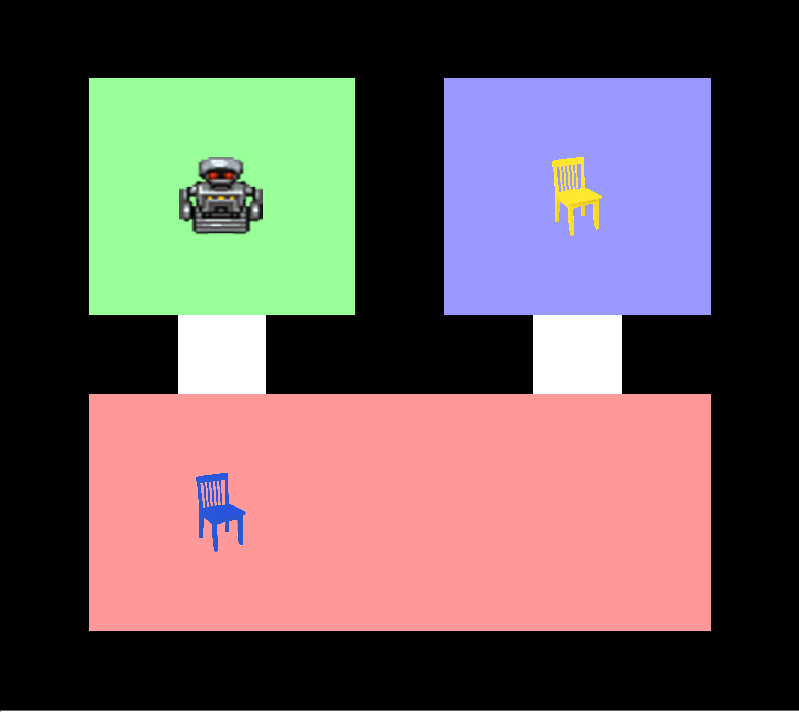
\includegraphics[width=0.7\columnwidth]{images/exampleFloor}
\caption{\small An example three-room layout with one robot and two chairs. The object references for the red (lower), green (upper left), and blue (upper right) rooms are $r_1, r_2,$ and $r_3$, respectively. The references for the yellow (upper) and blue (lower) chair are $c_1$ and $c_2$.
}
\label{fig:ef}
\end{center}
\end{figure}
In this section, we describe the overall execution and learning process of our approach. In the next section, we will detail our generative model of tasks, behavior, and language that enables these processes. As a running example, consider the initial state of our {\em Cleanup World} domain shown in Figure~\ref{fig:ef}. Cleanup World (inspired by Sokoban \cite{junghanns1997sokoban}) is a 2D grid world of various rooms connected by open doors. Rooms can also contain ``blocks'' that can be moved around. The robot moves using north-south-east-west actions. Moving into a location containing a block causes the block to move in the direction the agent is moving. If a wall or other item is in its immediate path, neither the agent nor the block moves. Cleanup World is represented as an OO-MDP consisting of four object classes: ${\tt ROBOT}$, ${\tt BLOCK}$, ${\tt ROOM}$, and ${\tt DOORWAY}$.
The propositional functions defined for the OO-MDP include ${\tt robotInRoom}({\tt ROBOT}, {\tt ROOM})$, and ${\tt blockInRoom}({\tt BLOCK}, {\tt ROOM})$, as well as propositional functions to indicate the color and type of rooms and blocks (e.g., ${\tt roomIsOrange}({\tt ROOM})$, ${\tt blockIsStar}({\tt BLOCK})$).

Figure~\ref{fig:execute} shows a flow chart of the execution process. To illustrate the steps of this process, considering the command ``take the yellow chair to the red room'' being given in the state shown in Figure~\ref{fig:ef}. Using Bayesian inference with the learned model, the most likely task for the state shown in Figure\ref{fig:execute} is the goal condition ${\tt blockInRoom}(b_1, r_1)$, because the command uses words for taking an object to a location, and because the selected objects satisfy the properties ${\tt roomIsRed}(r_1) \land {\tt blockIsYellow}(b_1) \land {\tt blockIsChair}(b_1)$, which would have a high probability of generating the English words in the command. Once the most likely task has been inferred, a standard plan and control problem is instantiated, in which the robot uses a planning algorithm to generate a policy and follows the policy in a closed loop fashion.\footnote{The policy does not have to be complete and can invoke replanning if it is more efficient to do so.} Our approach is independent of the planning algorithm: it can use any ``off-the-shelf'' planning algorithm appropriate for the domain, allowing our approach to apply to a large variety of robotics domains as long as enough of the state is observable to perform task grounding.

\begin{figure}
        \centering
        \begin{subfigure}[b]{\columnwidth}
                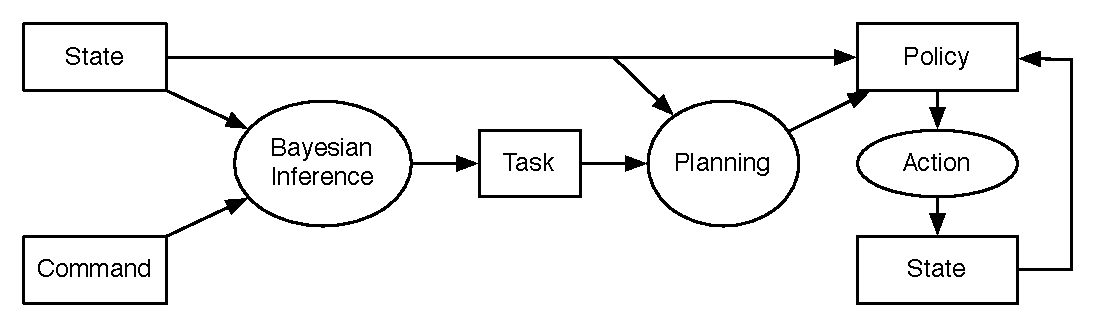
\includegraphics[width=\textwidth]{images/executeFlow}
                \caption{\small A flow chart of command execution.}
                \label{fig:execute}
        \end{subfigure}%
        \\
        \begin{subfigure}[b]{\columnwidth}
                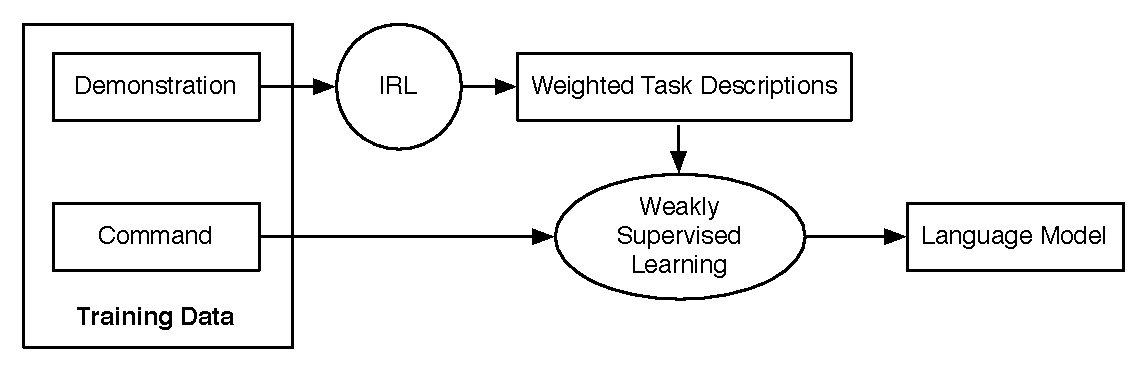
\includegraphics[width=\textwidth]{images/trainFlow}
                \caption{\small A flow chart of the training process.}
                \label{fig:learn}
        \end{subfigure}
        \caption{\small Flow charts for command execution and learning.}\label{fig:flow}
\end{figure}

Figure~\ref{fig:learn} shows a flow chart of the learning process for taking a dataset of demonstrations paired with commands and learning the parameters of a language model that ground language to latent task descriptions. Learning requires the set of OO-MDP propositional functions to which language is ground to be known in advance, but it does not require the natural language to be known in advance. Consider the previous command ``take the yellow chair to the red room'' in the role of a training instance, paired with a demonstration that starts in the initial state shown in Figure~\ref{fig:ef} and then follows the action sequence $SSSEEEENNWNNESSS$, where $N, S, E, W$ stand for north, south, east, and west, respectively. From this demonstration, inverse reinforcement learning (IRL) infers the probability that each possible task in the environment of the demonstration was the task being completed by the demonstration. The task with the goal ${\tt blockInRoom}(b_1, r_1)$ will have a very high probability compared to other tasks. This task has many possible descriptions based on the properties of the objects $b_1$ and $b_2$ to which language could be ground. In particular, one such task description is ${\tt blockInRoom}(b_1, r_1) {\tt roomIsRed}(r_1) \land {\tt blockIsYellow}(b_1) \land {\tt blockIsChair}(b_1)$. The set of all possible task descriptions for all tasks, weighted by the probability of their task being the intended one, form a set of weakly supervised labels for the training command and are used with a weakly supervised learning algorithm to train the language model parameters.

Our approach can easily incorporate different semantic language models. We investigate two language models---a bag-of-words (BoW) mixture model and
the IBM Model 2 (IBM2) used in statistical machine translation~\cite{brown90,brown93}---and use expectation maximization~\cite{dempster77} for training them with the weakly labeled commands. While other language
models that incorporate grammatical knowledge might yield better
performance and robustness, an advantage of these grammar-free models
is that they do not require any additional corpus training and can be
used with our task and behavior model as is. 

For these language models, semantic parsing through inference on a trained model was very fast, because the set of semantic interpretations was small compared to translating to another full natural language, for which IBM2 is typically used. The more demanding process of the command execution is planning, which will increase in complexity as the environment becomes more complex. However, since different planning algorithms may be used, this approach will scale to more complex environments as planning algorithms scale. 

Given the weakly labeled task descriptions, training the language models was also fast using the expectation maximization algorithm~\cite{dempster77} (see Section~\ref{sec:learnLang}). The primary computational cost lies in performing IRL for each demonstration. In our domain, performing IRL on a demonstration requires planning for all the finite possible tasks in the environment. As with command execution, this cost will scale to more complex environments as planning algorithms scale. In our tests, the number of possible tasks in the environment was not prohibitive. In domains with a very large number of tasks per environment, approximate inference or a scaffolding procedure in which the trainer iteratively trains the robot with simple environments may be beneficial. We leave this investigation for future work. 

\section{The Generative Model}
\begin{figure}[tbp]
\begin{center}
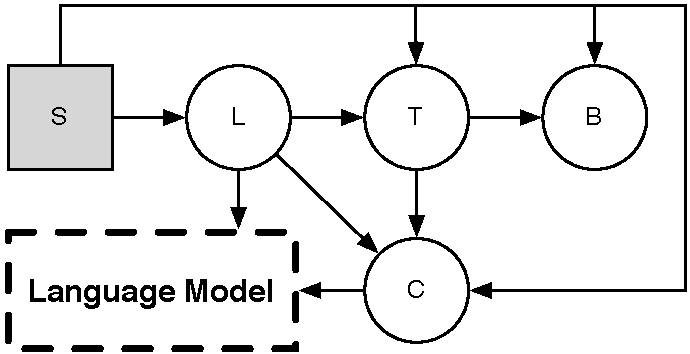
\includegraphics[width=.7\columnwidth]{images/taskModel}
\caption{\small The generative task model, with arrows indicating conditional probabilities. $S$ is the current state and is an input to the model. $L$ is the lifted task; $T$ is the grounded task; $B$ is the behavior of the agent; and $C$ is the object-binding constraints. The language model is a parameter of our overall generative model.}
%The generative task model, with arrows indicating conditional probabilities. $S$ is the current state and is an input to the model. $L$ is the lifted task, which specifies the kind of problem to solve. $T$ is the grounded tasks, which binds specific objects to the lifted task making for a well defined problem to solve. $B$ is the behavior the agent follows to complete task $T$. $C$ is the object-binding constraints, which specify properties about the bound objects in $T$ that a user might refer to in their language to specify the objects. The language model is a parameter of our overall generative model.}
% An arrow from $X\rightarrow Y$ indicates that $Y$'s probability distribution is conditionally dependent on $X$.}
\label{fig:tm}
\end{center}
\end{figure}
Our generative model of tasks, behavior, and language used for learning and command execution is shown in Figure~\ref{fig:tm}. It consists of an input initial state ($S$), a set of lifted tasks ($L$), a set of grounded tasks ($T$), a set of object-binding constraints ($C$), a set of behavior demonstrations/trajectories ($B$), and a language model that produces natural language commands and is dependent on the lifted task and binding constraints. A lifted task specifies the kinds of problems the agent can solve with propositional functions, but leaves the OO-MDP objects on which it operates as free variables; a grounded task binds a lifted task's free variables to specific objects in the world, thereby producing a well defined decision-making problem; object-binding constraints specify the set of possible properties of the grounded task's bound objects that a user might refer to in language; and a behavior trajectory is a sequence of states and actions taken by the agent. 
%In the rest of this section, we will describe these various components and their probability distributions in more detail. 
%We will refer to the same running example shown in Figure~\ref{fig:ef} discussed previously. 
%Note that the specific language model is a parameter of our overall model and learning algorithm, but we will describe two grammar-free models we investigated in this work: a Bag-of-Words mixture model and
%the IBM Model 2 used in statistical machine-translation~\cite{brown90,brown93}. 




%Our goal is to learn how to ground language to task descriptions represented as MDP reward functions indirectly from demonstrations of the tasks being carried out in the low-level action space. To perform this learning, we use a form of IRL to identify the set of likely tasks from each demonstration and use the identified tasks and their probability to perform weakly supervised learning of the language model. Once the grounding between language and tasks is learned, an agent can receive a command, ground it into a reward function, and then compute a policy to follow to complete the task using any ``off-the-shelf'' MDP planning algorithm.%

%To ground language to reward functions and perform IRL from demonstration to those possible reward functions, we introduce a generative model of factored reward functions, behavior, and language. More specifically, we assume that any {\em task} that a person may request can be represented as a reward function and corresponding terminal states (if it is a terminating task) defined with OO-MDP propositional functions. 
%Everything about the OO-MDP, except the task, is assumed to be known by the agent. Our generative model, shown in Figure \ref{fig:tm}, consists of an input initial state ($S$), a set of lifted tasks ($L$), a set of grounded tasks ($T$), a set of object-binding constraints ($C$), a set of behavior demonstrations/trajectories ($B$), and a language model that produces natural language commands and is dependent on the lifted task and binding constraints. A lifted task specifies the kinds of problems the agent can solve with propositional functions, but leaves the OO-MDP objects on which it operates as free variables; a grounded task binds a lifted task's free variables to specific objects in the world, thereby producing a well-defined decision-making problem; object-binding constraints specify the set of possible properties of the grounded task's bound objects that a user might refer to in language; a behavior trajectory is a sequence of states and actions taken by the agent. Note that the specific language model is a parameter of our overall model and learning algorithm. In the following section, we will discuss two grammar-free models that we successfully used to ground several tasks. In the rest of this section, we will describe these various components and their probability distributions in more detail. As a running example, we will refer to the example Cleanup World state shown in Figure \ref{fig:ef}. An example training instance in this example environment is the English command ``take the yellow chair to the red room'' which would be paired with the low-level action sequence $SSSEEEENNWNNESSS$, where $N, S, E, W$ stand for north, south, east, and west, respectively. Using IRL, the most likely task would be one that satisfies the goal ${\tt blockInRoom}(c_1, r_1)$, which has many possible object-binding constraints, such as ${\tt isRed}(r_1)$.


%\stnote{Can you provide an example of a training example?  Here's my stab:  ``For example, the robot learns from language, such as ``Move the blue block to the beige room'' paired with low-level action sequences such as NNSSEESSS.  We use IRL to map between the low-level action sequence and abstract reward functions, such as ``moveBlock(room1, room2).''''  (I know this example isn't using the right notation but I thought I would take a stab and then James can fix up the notation if you like the idea.  I think it would help to make the learning problem more concrete sooner before going into all the details.  And also emphasize that it's hard.)}


\subsection{Lifted Tasks}
The set of possible lifted task definitions is provided by a designer and represents the kinds of tasks an agent could conceivably carry out in an environment. Specifically, each lifted task is a factored reward function defined as a logical expression of OO-MDP propositional functions with the parameters of the propositional functions set to free variables. In our example environment (Figure \ref{fig:ef}), a reward function for the task of taking a ``block'' object (e.g., chair) to a room is:
\begin{equation}
\label{eq:liftedrf}
{\cal R}(s, a, s') = \begin{cases}
1 & \mbox{if } {\tt blockInRoom}^{s'}(?b, ?r) \\
0 & \mbox{otherwise}
\end{cases},
\end{equation}
where $s'$ is the outcome state for the agent after taking action $a$ in state $s$, ${\tt blockInRoom}^{s'}$ is a propositional function evaluated in state $s'$, $?b$ is a free variable that can be grounded to any movable block object in the environment, and $?r$ is a free variable that can be grounded to any room in the environment. 
If a task is goal-directed, then the reward function will also be paired with a similar set of termination conditions.

The prior probability distribution on the set of lifted tasks is assumed to be uniform over the set of lifted tasks that are {\em permissible} in an input state. A lifted task is permissible in an input state if there exists at least one object of each object class required by the free variables in the lifted task. For example, if the input state has no block objects present, then lifted task \ref{eq:liftedrf} is {\em not} permissible in the state. 
%Using lifted tasks enables our system to generalize its learned knowledge across different environments because it infers an abstract description of the person's goals that is not specific to the low-level action sequence that it must observe or generate.

\subsection{Grounded Tasks}
A grounded task ($T$) is dependent on the lifted task and input state and is an assignment of objects in the input state to each of the free variables in the lifted task. For example, given the input state shown in Figure \ref{fig:ef}, an object assignment to lifted task \ref{eq:liftedrf} that represents the task of the robot taking the yellow chair to the red room is $?b:=c_1$ and $?r:=r_1$. The probability distribution of grounded tasks is uniform over the set of possible variable assignments for the lifted task. In goal-directed tasks, only tasks that are not satisfied in the initial state are considered.
Because our task model starts with lifted tasks that are defined with free variables and then finds all possible groundings in the current input state, it generalizes to environments with any number of objects present.

\subsection{Object-Binding Constraints}
If language was only dependent on the lifted task, it would be impossible for the agent to determine which of the possible grounded tasks for an input state was the intended task from a command.
Object-binding constraints ($C$) are logical expressions that extend a lifted task and on which language is dependent, enabling the agent to resolve grounding ambiguity. 
% For example, we can infer from the command ``take the yellow chair to the red room,'' that the grounding of lifted task \ref{eq:liftedrf} should satisfy the constraints ${\tt isYellow}(?b) \land {\tt isRed}(?r)$
For example, the command ``take the yellow chair to the red room'' indicates that a grounding for lifted task \ref{eq:liftedrf} should satisfy the constraints ${\tt isYellow}(?b) \land {\tt isRed}(?r)$.

The probability distribution of object constraints given a grounded task, lifted task, and input state is uniform across the set of possible additional logical constraints that are true in the input state for the given variable assignments in the grounded task. For example, if $?b$ is assigned to $c_1$ in the grounded task, ${\tt isYellow}(?b)$, is a possible constraint since it is true in the initial state for $c_1$, but ${\tt isBlue}(?b)$ is not.

\subsection{Behavior}
A \emph{behavior trajectory} is a sequence of state--action pairs that the agent can experience from an input state and is conditionally dependent on the grounded task and input state. The conditional probability of the behavior, given the task, is formulated by treating each action selection in each state of the trajectory as an independent event and by defining the action-selection probability distribution as a noisy version of the policy computed by an ``off-the-shelf'' planning algorithm. Following maximum likelihood inverse reinforcement learning~\cite{babes11}, we use a Boltzmann distribution over the optimal Q-values as the noisy policy. The probability of any behavior trajectory $b$ (of length $N$) given task $t$ is defined as:
\begin{equation}
\label{eq:trajProb}
\Pr(b | t) = \prod^N_i \pi_t(s_i, a_i), 
\end{equation}
where $(s_i, a_i)$ is the $i$th state--action pair in behavior trajectory $b$ and $\pi_t(s_i, a_i)$ is the noisy policy distribution under task $t$ (the probability of taking action $a_i$ in state $s_i$ when the task is task $t$). 

%Given the optimal Q-values for an MDP, the Boltzmann policy distribution is defined as
%\begin{equation}
%\pi(s, a) = \frac{e^{\frac{Q(s, a)}{\tau}}}{\sum_{a'}e^{\frac{Q(s, a')}{\tau}}},
%\end{equation}
%where $\tau$ is a temperature parameter. Higher temperatures make the model less sensitive to suboptimal actions taken in the demonstration, but less discriminative between different tasks. Lower temperature values are more discriminative, but are also more sensitive to error when the demonstration contains suboptimal actions. 

For goal-directed tasks, we add a virtual ``terminate'' action to the MDP that must be executed to actually terminate the task; this virtual terminate action is added to the end of observed trajectories. The inclusion of a terminating action more strongly differentiates between tasks where the optimal trajectory for one task is a subsequence of the optimal trajectory for another. For example, an optimal trajectory for going to the red room is a subsequence of an optimal trajectory for going to the blue room (in Figure \ref{fig:ef}), but since it is not expected for the agent to terminate in the red room if the task is to go the blue room, terminating in the red room makes it more likely for the trajectory to be generated by a ``go to the red room'' task.

%If the task is a terminating goal-directed task, this conditional probability formalism may inappropriately assign equal probability to a trajectory under two different tasks if the optimal policy for one is a subset of the other. For example, consider a home in which going to the dining room requires going through the living room. A demonstration of a task for going to the living room will be assigned the same probability under both the living room  and dining room task, because the policy for the states in the demonstration would be identical. To address this limitation, we augment the MDP action set to include a special terminating action that must be executed for the agent to end the task and receive the goal reward. The demonstration is then augmented to include the agent executing the terminate action at the end. In our previous example, a demonstration of going to the living room would not produce equal probability for the dining room task because it would be suboptimal for the agent to terminate the task before it accomplishes its goal.


%The task model presented above can be combined with any language model as long as its probability distributions can be made dependent in some way on the lifted task and object binding constraints. The notation $\Pr(e | l, c)$ is used to represent the probability of a natural language command $e$ given lifted task $l$ and object binding constraints $c$; this probability is assumed to be defined by the specific language model used. Given the language model, we have a complete generative model from tasks to behavior and language, and can perform learning from a dataset of demonstrations and natural language command pairs using any parameter inference algorithm, such as Expectation Maximization (EM) \cite{dempster77}. The agent can then infer the most likely task given a natural language command, plan behavior to complete it, and execute the plan. Specifically, the probability of task $t$ given natural language command $e$ and input state $s$ is:
%\begin{equation}
%\Pr(t | e, s) \propto \sum_l \Pr(l | s) \Pr(t | s, l) \sum_c \Pr(c | s, l, t) \Pr(e | l, c).
%\end{equation}




%Mapping natural language commands to reward functions is especially useful, because it allows the person giving the command to avoid having to give detailed action-level instructions about how to complete a task. Instead, once the reward function is known, the agent can plan out how accomplish the task itself. For instance, if we wanted a human assistant to take a bunch of books to another room, we wouldn't give instructions about how to pick up the books, carry them, or anything else at that level of detail. We'd simply tell them to take the books to the desired room. Furthermore, we wouldn't expect to have to give a human assistant different commands if we spoke to them in different rooms, because the goal would be the same. By mapping commands to reward functions, we can given autonomous agents similarly high-level commands that they can turn into complex behavior depending on the situation.

%We next delve more deeply into the model that relates language and tasks.
% zzz ML: should make a note to thank Eugene for IBM Model 2 if the paper is accepted.

\section{Language Models} 
\label{section:lm}

We investigated two grammar-free language models for use with our task model: a BoW model and IBM Model 2.

\subsection{Bag-of-Words}
In the bag-of-words (BoW) model, commands are treated as an unordered bag of words generated from a mixture model of semantic components, similar to previous topic modeling approaches \cite{McCallum:1999vn}. The semantic components, given a lifted task and object-binding constraints, include (1) the set of propositional function names included in the task and binding-constraint expressions, (2) the object class names of the arguments of the propositional functions, and (3) a constant symbol ($\#$) that acts as a catchall for words not explicitly related to a semantic component. For example, lifted task \ref{eq:liftedrf} coupled with the constraint ${\tt isRed}(?r)$ would have the semantic components ${\tt blockInRoom}, {\tt isRed}, {\tt BLOCK}, {\tt ROOM}$, and $\#$. The probability that any semantic component is selected to generate a word is proportional to its frequency of appearance in the task and binding-constraint expressions.

The parameters of the BoW model are the conditional probabilities that any word will be generated from a given semantic component. Therefore, the probability of a command ($e$) given a lifted task ($l$) and object-binding constraints ($c$) is
\begin{equation}
\Pr(e | l, c)  = \prod_{w \in e} \left[ \sum_v \Pr(v | l, c) \theta_{vw} \right]^{K(w, e)},
\end{equation}
where $\theta_{vw}$ is a parameter specifying the conditional probability that the natural language word $w$ is generated given semantic component $v$, and $K(w, e)$ is the number of times that word $w$ appears in command $e$.

%A limitation of the BoW model is that, because it does not account for word order or structure, it cannot disambiguate which words in a command apply to which object. For example, for the command ``take the blue chair to the red room,'' BoW would not be able to disambiguate whether ``blue'' refers to the chair or the room (and similarly for the word ``red'').

%The Bag-of-Words (BoW) language model 
%is similar to the topic modeling approach used by McCallum \shortcite{McCallum:1999vn}, in which words are distributed according to a mixture of topics and a document is generated by selecting a topic with some mixture weight, generating a word from the topic's word distribution, and then repeating the process. In our BoW model (Figure~\ref{fig:bowm}), we replace the role of topics with semantic components of the lifted task and object binding constraints, generating words as a mixture model of those semantic components. 
%\begin{figure}[tbp]
%\begin{center}
%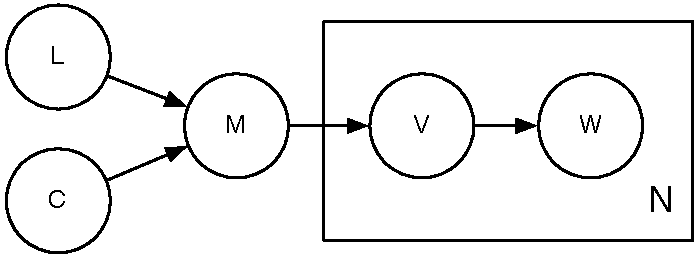
\includegraphics[width=.7\columnwidth]{images/bowModel}
%\caption{The Bag-of-Words model.}
%\label{fig:bowm}
%\end{center}
%\end{figure}%

%Random variable $M$ is assigned a frequency vector of the semantic components that appear in the lifted task and object binding constraints, consisting of the names of propositional functions and the object class names of the parameters of the propositional functions; a special constant referred to by the symbol `\#' is also always assumed to appear once. For instance, for the lifted task in Equation \ref{eq:liftedrf} and object binding constraint ${\tt isRed}(?r)$, the corresponding value assigned to variable $M$ would be: 
%\small
%\[
%\langle \#=1, {\tt blockInRoom}=1, {\tt isRed}=1, {\tt BLOCK}=1, {\tt ROOM} = 2 \rangle .
%\]
%\normalsize
%Normalizing the frequency of each semantic component defines the conditional probability that a semantic component will be selected ($\Pr(v | m)$); any semantic component not in the semantic component frequency vector $m$ is assigned zero probability. For a command of length $n$, a semantic component will be selected $n$ times, each time generating a natural language word according to a multinomial word distribution for each semantic component. Therefore, the conditional probability of any natural language command $e$ is:
%\begin{equation}
%\Pr(e | m)  = \prod_{w \in e} \left[ \sum_v \Pr(v | m) \theta_{vw} \right]^{K(w, e)},
%\end{equation}
%where $\theta_{vw}$ is a parameter specifying the conditional probability that the natural language word $w$ is generated given semantic component $v$, and $K(w, e)$ is the number of times that word $w$ appears in command $e$.%

%For this model, the parameters $\theta$ can be learned using  EM.
%At each iteration, the parameters
%are updated using the formula $\theta_{vw} = \frac{\hat{N}(v, w)}{\hat{N}(v)}$, where $\hat{N}(x)$ is the expected number of times that $x$ appears in some dataset. For a dataset consisting of pairs of demonstration behavior and natural language commands ($D = \{(b_1, e_1) ... (b_{|D|}, e_{|D|})\}$), these values are computed as follows:
%\tiny
%\begin{align}
%\hat{N}(v, w) &= \sum_i\frac{K(w, e_i) \sum_m \Pr(v | m) \theta_{vw} \Pr(e_i-w | m) U(m, b_i | s_i)}{\sum_m \Pr(e_i | m) U(m, b_i | s_i)} \\
%\hat{N}(v) &= \sum_i \frac{\sum_{u} K(u, e_i) \sum_m \Pr(v | m) \theta_{vu} \Pr(e_i-u | m) U(m, b_i | s_i)}{\sum_i \sum_m \Pr(e_i | m) U(m, b_i | s_i)},
%\end{align}
%\normalsize
%where $\Pr(e_i-w | m)$ is the probability of the command $e_i$ given the semantic component frequency vector $m$ if one occurrence of the word $w$ were removed from the command $e_i$, and
%\tiny
%\begin{equation}
%U(m, b | s) = \sum_{l, t, c} \Pr(l | s) \Pr(t | l, s) \Pr(b | s, t) \Pr(c | s, l, t) \Pr(m | l, c).
%\end{equation}
%\normalsize

\subsection{IBM Model 2}

%SM I made this more high level. The prose of describing the IBM Model 2 I think is to detailed,  ideally would be to give the general IBM Model 2 for MT in its noisy-channel formulation, so the similarities can be seen directly. 
IBM Model 2 (IBM2) \cite{brown90,brown93} is a word-based statistical machine-translation model. In statistical machine translation, the task is to translate a sentence from a source language $f$ (e.g., French) to a target language $e$ (e.g., English). Our task corresponds to the problem of translating from an English command $e$ to its corresponding machine-language command $m$. 

We integrate IBM2 into our task and behavior model by using the lifted task and object-binding constraints to deterministically generate a machine-language command $m$ and then generate the natural language command $e$ from $m$ in the standard IBM2 fashion. 
A machine-language command ($m$) is generated from a lifted task ($l$) and object-binding constraints ($c$) by first adding each semantic component in $l$
to $m$ in the order that the components appear. Next, the same is done for the components of $c$. For example, the lifted task in Equation~\ref{eq:liftedrf} and object-binding constraint ${\tt isRed}(?r)$ would generate the machine-language command ``\# blockInRoom block room isRed room,'' where \# is the constant symbol that IBM2 always assumes to be present at the start of an expression. The probability of a natural language command ($e$) given the machine-language command ($m$) is defined as:

{\small
\begin{equation}
\vspace{-1em}
\Pr({\mathbf e} | {\mathbf m}) = \eta(n_e | n_m) \sum_{\mathbf a} \prod_j^{n_e} q(a_j | j, n_m, n_e) r(e_j | m_{a_j}),
\end{equation}
}

\noindent where $\eta(n_e | n_m)$ is the parameter specifying the probability that a machine-language command of length $n_m$ %$m$'s length 
would generate a natural language command of length $n_e$; %$e$'s length;
${\mathbf a}$ is a possible alignment from natural language words to machine-language words; $q(a_j | j, n_m, n_e)$ is the alignment parameter specifying the probability that the natural language word in position $j$ would be aligned with the machine-language word in position $a_j$ for a machine-language command of length $n_m$ and natural language command of length $n_e$;  and $r(e_j | m_{a_j})$ is the translation parameter specifying the probability that natural language word $e_j$ would be generated from machine-language word $m_{a_j}$. The number of alignments (${\mathbf a}$) is typically very large, so in practice we estimate the value using sampling. 
 

%The probability of any possible machine-language command can be computed from the demonstrations in the data:
%\tiny
%\begin{equation}
%\Pr(m | s, b) = \frac{\sum_{l,t,c} \Pr(l | s) \Pr(t | s, l) \Pr(b | s, t) \Pr(c | s, l, t) \Pr(m | l, c)}{\sum_{l,t} \Pr(l | s) \Pr(t | s, l) \Pr(b | s, t)}.
%\end{equation}
%\normalsize
%We use a modified EM algorithm in which each natural language command in the dataset is paired with all machine-language commands with non-zero probability given the behavior trajectory, and the counts computed by the EM algorithm are weighted by that probability.
%The resulting weakly supervised learning algorithm is shown as pseudocode in the the supplementary document.
%%shown in Algorithm \ref{alg:wsmt}.
%The method re-estimates the $q$ and $r$ parameters iteratively. In each iteration, it loops through each non-zero probability machine-language command for each data instance in the dataset. For each of those machine-language commands, it matches each natural language word with each machine-language word (including the constant word), updating the relevant expected counts for the $q$ and $r$ parameters by a value $\delta$, where $\delta$ represents the machine-language-command-weighted probability that a given natural language word in a given position of the natural language command would have been generated by a given machine-language word in a given position of a machine-language command. Formally:
%\small
%\begin{equation}
%\delta(i, j, u, m) = \Pr(m | s_i, b_i) \frac{q(u | j, n_m, n_i) r(e_j | m_u)}     {\sum_v q(v | j, n_m, n_i) r(e_j | m_v)}.
%\end{equation}
%\normalsize
%After the expected counts have been estimated for the whole dataset, the $q$ and $r$ parameters are updated according to them and the process repeats. Note that this algorithm does not update the $\eta$ parameter, which specifies the probability that a natural language command of certain length is generated by a machine-language command of a certain length. Because this parameter does not depend on the $q$ or $r$ parameters it is set once according to:
%%SM shouldn't n and k be instead n_e and n_m to match equation 9? 
%\begin{equation}
%\eta(n_e | n_m) = \frac{\sum_i I(e_i, n_e) \sum_m I(m, n_m) \Pr(m | s_i, b_i)}{\sum_i \sum_m I(m, n_m) \Pr(m | s_i, b_i)},
%\end{equation}
%where $I(x, y)$ is an indicator function that returns one when the length of command $x$ is $y$ and zero otherwise.

\subsection{Learning Language Model Parameters}
\label{sec:learnLang}
Given a dataset of trajectory demonstration and natural language command pairs, the language model parameters can be learned through weakly supervised learning. 

When the task and behavior model is paired with the BoW language model, we use a standard Bayesian Network expectation maximization (EM) algorithm \cite{dempster77} to iteratively update the BoW model's word generation parameters. 
%Each iteration, the total expeced number of occurences of each semantic component and semantic component word pair is estimated. For a dataset of training command ($e_i$) and trajectory ($b_i$) pairs, the expected occurences of semantic component $v$ and semanic component word pair $v,w$ is
%\tiny
%\begin{align*}
%\hat{N}(v, w) &= \sum_i \frac{K(w, e_i) \sum_{l,c} \Pr(v | l,c) \theta_{vw} \Pr(e_i-w | l,c) U(l, c, b_i | s)}{\sum_{l,c} \Pr(e_i | l,c) U(l, c, b_i | s)} \\
%\hat{N}(v) &= \sum_i \frac{\sum_{u} K(u, e_i) \sum_{l,c} \Pr(v | l,c) \theta_{vu} \Pr(e_i-u | l,c) U(l,c, b_i | s)}{\sum_{l,c} \Pr(e_i | l,c) U(m, b_i | s_i)},
%\end{align*}
%\normalsize
%where $\Pr(e_i-w | l,c)$ is the probability of the command $e_i$ given lifted task $l$ and constraints $c$ if one occurrence of the word $w$ were removed from $e_i$, and
%\small
%\begin{equation}
%U(l, c, b | s) = \sum_{t} \Pr(l | s) \Pr(t | l, s) \Pr(b | s, t) \Pr(c | s, l, t).  
%\end{equation}
%\normalsize
%Parameters are then updated according to $\theta_{vw} = \frac{\hat{N}(v, w)}{\hat{N}(v)}$.

In classic IBM2 parameter learning, EM is used on a training dataset consisting of pairs of natural language expressions (e.g., French and English), often with a ``bake-in'' period, during which only translation parameters are updated, followed by a normal learning phase during which translation parameters and alignment parameters are updated. We follow the same approach here, except in our case, we have pairs of machine language commands and English commands, and the contribution of the expectation of machine language commands is weighted by the probability of being generated given the demonstration (see Section~\ref{sec:el}). The probability of any machine-language command ($m$) given a trajectory ($b$) and initial state ($s$) is:

{
\footnotesize
\begin{equation}
\vspace{-1em}
\begin{split}
& \Pr(m | s, b) = \\ & \frac{\sum_{l,t,c} \Pr(l | s) \Pr(t | s, l) \Pr(b | s, t) \Pr(c | s, l, t) \Pr(m | l, c)}{\sum_{l,t} \Pr(l | s) \Pr(t | s, l) \Pr(b | s, t)}.
\end{split}
\end{equation}
}


%In our dataset, we have pairs of trajectory and natural language commands, so we use a modified version of the classic IBM2 EM algorithm where we convert each trajectory into a set of possible machine-language commands weighted by the probability that each machine-language command would be generated given the trajectory. Then, the standard IBM2 EM update rules are performed on the pairs of machine-language and natural language commands, except the contribution of each pair is weighted by the probability of that machine-language command having been generated by its associated trajectory. The probability of any machine-language command ($m$) given a trajectory ($b$) and initial state ($s$) is%

%{
%\footnotesize
%\begin{equation}
%\vspace{-1em}
%\begin{split}
%& \Pr(m | s, b) = \\ & \frac{\sum_{l,t,c} \Pr(l | s) \Pr(t | s, l) \Pr(b | s, t) \Pr(c | s, l, t) \Pr(m | l, c)}{\sum_{l,t} \Pr(l | s) \Pr(t | s, l) \Pr(b | s, t)}.
%\end{split}
%\end{equation}
%}

\noindent A similar approach could be used for training the parameters of other language models.

\section{Experimental Results}
To empirically validate our approach, we collected example language for the ``Cleanup World'' from two different sources: an Amazon Mechanical Turk (AMT) user study and an ``expert'' who is an author of this paper. Different experiments were run for the AMT language source and the expert source. In the AMT study, we asked users to provide example commands for a smaller range of tasks, but used more abstract object representations and unusual color choices to elicit more variety in the command descriptions. In the expert study, we evaluated a larger range of tasks and environments but with fairly clean expressions of the language. The details of the various experiments run with each study are explained below. We also show how we can take the language model learned from the AMT study, recreate the Cleanup World domain on an actual mobile robot, and successfully transfer the learned model so that the robot correctly interprets the commands, even though the robot has a different action space than the simulated robot used for training.

%Cleanup World (like Sokoban \cite{junghanns1997sokoban}) is a 2D grid world of various rooms connected by open doors. Rooms can also contain ``blocks'' that can be moved around. The robot moves using north-south-east-west actions. Moving into a location containing a block causes the block to move in the direction the agent is moving. If a wall or other item is in its immediate path, neither the agent nor the block moves. Cleanup World is represented as an OO-MDP consisting of four object classes: ${\tt ROBOT}$, ${\tt BLOCK}$, ${\tt ROOM}$, and ${\tt DOORWAY}$. %The agent is defined by $x$ and $y$ position attributes. Blocks are defined by position attributes, a color attribute, and a shape attribute. The room and door objects are defined by attributes describing their rectangular bounding box (top, left, bottom, right), and the room object also has a color attribute. 
%The propositional functions defined for the OO-MDP include ${\tt robotInRoom}({\tt ROBOT}, {\tt ROOM})$, and ${\tt blockInRoom}({\tt BLOCK}, {\tt ROOM})$, as well as propositional functions to indicate the color and type of rooms and blocks (e.g., ${\tt roomIsOrange}({\tt ROOM})$, ${\tt blockIsStar}({\tt BLOCK})$).

In both studies, the Boltzmann policy parameter $\tau$ was set to $0.005$. Since we knew the task that the training commands were meant to describe, performance was measured using leave-one-out (LOO) cross validation on the collected training examples; a prediction was considered correct if the interpretation of the reward function resulted in behavior that achieved the actual goal. 

For a baseline, we compared to a model that grounds language to actions rather than tasks. Because the order of the actions is important, we always paired the baseline with the IBM2 language model. When training the IBM2 model, the action sequence in the demonstration is converted into a machine-language sentence in which each word is the name of the action. Note that the action-grounding learning problem is in some sense easier than training the task model, since the action sequence is always directly observed in the demonstration, whereas in our task grounding model, IRL is needed to perform weakly supervised learning. Inferring an action sequence from a command would generally require searching the action sequence space and finding the most likely sequence from the command or at least using it to bias a planning algorithm's search, similar to the work of \citet{chen11}. However, we simplify this inference problem greatly by allowing the action-grounding model to exploit our task model. Specifically, when inferring an action sequence for a command, the only valid action sequences permitted are those that solve one of the possible grounded tasks; the baseline always chooses the most likely of the possible sequences.







\subsection{AMT Dataset}
In the AMT study, we considered two different lifted tasks: the robot going to a specific room and the robot moving a block to a specific room. To collect natural language instructions for different grounded versions of these tasks, we presented Turkers on AMT animated images showing either the robot moving to a room of a specific color or moving a star block to a room of a specific color. An example image from the animation is shown in Figure \ref{fig:animation}.
\begin{figure}[tp]
\begin{center}
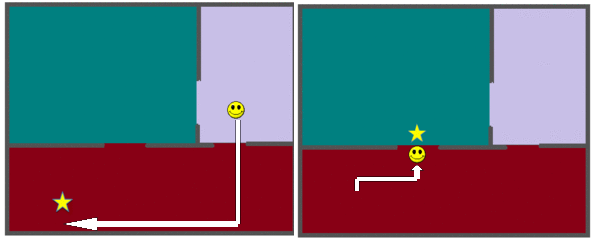
\includegraphics[width=\columnwidth]{images/map1_2a}
\caption{\small An example task to take a star to a room shown to users on AMT. The left frame shows the initial state and the path to the star; the right frame shows the path from there to the end state. (In the actual study, users were shown a single animated image without arrows.)}
%In the animation, the agent was shown to move along the path of the arrows.}
\label{fig:animation}
\end{center}
\end{figure}
%We chose to use ambiguous colors for the rooms in our visual representation to elicit different verbalizations for the different colors. 
To prevent contamination of the commands we received, we never provided users with any example commands. 

After removing sentences that did not follow the instructions or were provided by users who did not understand the labeling task that we were asking them to perform, we obtained a dataset of 240 instances. In a final system used by individual users iteratively training a robot, they would understand the task they were trying to train the robot to follow, so we do not expect similar command removal to be necessary.

The goal of our work is to be able to give autonomous agents high-level commands that leave the details of how to complete the task as a problem for the agent to solve. However, most of the natural language commands we received included some high-level details of the path the robot followed (e.g., subgoals), rather than only describing the task goal. 
For example, one such command was ``go through center opening into beige enclosure and get behind star and push it into opening of orange enclosure.'' 
Although this data is interesting because it tests our model's performance on language that it was not intended to model, a dataset that better reflects the problem we were trying to solve is also useful for comparison. Therefore, in addition to this source dataset, we  created a simplified version that omits the text that is extraneous to the task description. 
For instance, the previous example became: ``go through center opening and get behind star and push it into opening of orange enclosure.'' 
The average command lengths (in words) were $13.57$ and $8.87$ in the original and simplified datasets, respectively. We tested results on both the original dataset and this simplified version.

In the training data we gathered from users, the room layout was always the same; however, one of the advantages of our approach is that commands can generalize to novel environments. To demonstrate the ability for our approach to generalize to new environments, we created a third dataset in which we used LOO cross validation for the language on the original (unmodified) dataset and tested each command on three different novel environments. Note that these different environments were not merely a different spatial arrangement of the rooms compared to the training dataset; the environments also had different initial conditions for the agent not seen in the training environment, which results in a different set of propositional functions being true in the initial state. As a consequence, our task model could perform worse if, during training, it overfit the object-binding constraints to inappropriate features. We refer to this dataset as the {\em novel environment} (NE) dataset.

%In our analysis, we compare performance on both the original dataset and the simplified version. 
% SM can we give the average number of words per command in each of the datasets?
% JM done.

%if the most likely grounded task inferred from a natural language command was the actual grounded task.
% zzz ML: Would it make sense to change that to something like ``if the interpretation of the reward function results in behavior that achieved the actual goal''?

The LOO accuracy for each grounding model (task and action) and the paired language model (BoW and IBM2) on each variant of the dataset is shown in Table \ref{tab:res}. Note for comparison that if the agent randomly selected a permissible grounded task, it would achieve an expected accuracy of 37.5\% in the simplified and original dataset and 33.3\% accuracy in the NE dataset. 


%Note for comparison that if the agent randomly selected a grounded task from the set of permissible tasks in the test environment that were not already satisfied in the initial state, the expected accuracy would be 37.5\%.
On the simplified dataset, task grounding with both BoW and IBM2 performed well and comparably (according to a chi-squared test, BoW and IBM2 are not statistically different; $p = 0.54$). However, while action grounding was able to perform better than randomly guessing, it did not perform as well as BoW or IBM2; the difference was statistically significant ($p < 0.001$ on a chi-squared test with all three groups).

On the original dataset, task grounding performance dropped for both language models, although BoW's drop in performance was much greater than IBM2's drop in performance and of the two, only BoW's drop in performance was statistically significant ($p < 0.01$ and $p = 0.07$ for BoW and IBM2's decrease in performance, respectively). The action grounding baseline performed identically to its performance on the simplified dataset and is reasonably comparable to task grounding using IBM2.

On the NE dataset, both task models were able to successfully generalize from the training data to the novel environments, achieving nearly the same performance as its performance on the original dataset for the corresponding language model. In contrast, the action grounding baseline completely failed to generalize from its training data, achieving a performance worse than what would be expected from randomly choosing tasks.

%All three models performed well on the simplified dataset. Although BoW had a slightly higher accuracy, the differences between it and IBM2 were not found to be statistically significant ($p > 0.5$ in a chi-squared test).  The performance of both models was lower on the original full dataset than on the simplified dataset, which was expected since the original dataset had language that our task model was not designed to reflect. However, IBM2's performance only dropped by $7.15\%$ (which was not a statistically significant drop; $p > 0.07$), whereas BoW dropped by $30.75\%$ (which was a statistically significant drop; $p < 10^{-11}$). The difference in performance between the models on the original dataset was highly statistically significant ($p < 0.00001$).

% zzz possibly remove the paragraph below to save space.
%IBM2's superior performance to BoW on the original dataset was expected, because the original dataset often included instructions with many qualifiers. For instance, users described the agent's progress through various rooms and often remarked on the color of that room. For the BoW model, having multiple colors specified in the command made it impossible to disambiguate which color was associated with each semantic component, since the BoW model does not reason over any structure of the sentence. In contrast, in IBM2, the word position influences its association with each semantic word, which enabled IBM2 to pull out the parts of the text that were relevant to the task description. These results indicate that while BoW is effective for simple commands in which the words themselves are fully representative of the task, IBM2 should be preferred for commands in which the structure of the sentence matters.

To demonstrate that task grounding with IBM2 successfully learned reasonable groundings of English words, we extracted IBM2's translation parameters after it had finished training on the original dataset. The most likely English words generated from the semantic word ``robotInRoom'' (which was associated with the lifted ``go to room" task), were ``walk," ``through," ``move," ``go," and ``from."  ``From" and ``through" occurred because in ``go to room" tasks, users often described {\em from} which room to leave and often commanded the robot to go {\em through} a door to the goal room. For example, one of the commands provided was ``walk through doorway from orange room to beige room."

%The most likely English words to be generated from the ``block" semantic word were: ``into" and ``star;" the former because comamds often specified pushing the block into a room and the latter because the blocks were star shaped.

Since the color of rooms was typically used to describe the goal room of both lifted tasks, the words associated with it are especially relevant. The ``roomIsOrange" semantic word was mostly likely to generate the words ``red" and ``orange;" ``roomIsTan" was most likely to generate the words ``tan" and ``beige;" and ``roomIsTeal" was most likely to generate ``green" and ``blue."



\begin{table}[tb]
\begin{center}
\begin{tabular}{@{}lrrr@{}} \toprule
Grounding Model & Simplified Dataset & Original Dataset & NE Dataset \\ \midrule
 Task (BoW) & {\bf 83.75\%} & 53.75\% & 51.80\%\\ 
 Task (IBM2) & 81.25\% & {\bf 74.16\%} & {\bf 73.33\%} \\ 
 Action (IBM2) & 69.58\% & 69.58\% & 21.94\% \\\bottomrule
\hline
 \end{tabular} 
 \caption{\small LOO accuracy for the AMT datasets.}
 \label{tab:res}
\end{center}
\end{table}


%Between the the expert and AMT datasets we found that our approach can be used to successfully training a language model that can be used to ground language. Overall, the BoW language model seems like it will only be successful when commands are very simple, whereas IBM2 can handle more complex commands and may continue to improve with more data. %Exploring grammer-based models in the future may yield even better approaches. %We next compare to work related to our language grounding problem.


\subsection{Expert Dataset}
The expert dataset includes three kinds of goal-directed lifted tasks: one for going to a room; one for taking a block to a room; and one for taking a block to a room and then going to another room. Environments had either one or two blocks present, which could be either a chair or a bag, and three rooms whose colors varied between environments. The dataset consisted of many different verbal descriptions of tasks, which also resulted in different necessary object-binding constraints that would need to be inferred. For example, some expressions took the form of ``move the bag to the blue room,'' which requires object-binding constraints for the shape of the block (bag) and the color of the destination room. Another example is ``move bag to the room with chair,'' which requires inferring object-binding constraints for the shape of the target block, and a ${\tt blockInRoom}$ and a block-shape propositional function to disambiguate the target room. Different commands also had variable levels of specificity. For example, some included information that was not necessary to infer the correct task, such as ``push chair from blue room to red room,'' in which specifying the color of the room in which the chair {\em initially} resides (blue) is unnecessary when there is only one chair. We also included commands that could not be modeled with the propositional functions defined. For example, the command ``go to left room'' is not representable because there are no propositional functions defined that indicate the relative spatial position of the rooms.% and the color of the the ``left'' room can vary between environments, which means ``left'' cannot act as a proxy for a color.

A strength of our framework is that different demonstrations of a command, even suboptimal ones, can be given and still provide meaningful information. In our dataset, we have $35$ additional instances of a command given in the same environment, but with a different demonstration. However, to ensure that the LOO evaluation is always inferring behavior from either a novel command or a novel environment, we also created a version of the dataset that did not include any duplicate commands unless they were given in a different environment. We will refer to the dataset without multiple demonstrations in the same environment as {\em expert} and the dataset with multiple demonstrations as {\em expert-MD}. The expert dataset has $118$ instances, with $104$ unique commands ($14$ of the commands are the same as another, but are given in a different environment); expert-MD has $153$ instances. %Because the dataset consists of mostly novel commands, good performance requires that the language model be able to transfer what it's learned between commands.

The LOO performance of the expert datasets is shown in Table \ref{tab:res_e}. As a baseline, if the agent randomly selected a possible grounded task, it would have an expected performance of $8.7\%$ and $8.6\%$ for the Expert and Expert-MD datasets, respectively. On both the Expert and Expert-MD dataset, our task model with IBM2 performed the best and these differences were statistically significant ($p = 0.013$ on a chi-squared test with all three groups). Furthermore, IBM2 performed better on Expert-MD than Expert (and the differences were statistically significant with $p = 0.011$), whereas BoW and Action Grounding did not improve performance by any significant amount, suggesting that even better performance with task grounding with IBM2 may be possible with additional data, even if that data uses different demonstrations than prior examples. 


\begin{table}[tb]
\begin{center}
\begin{tabular}{@{}lrr@{}} \toprule
Grounding Model & Expert & Expert-MD \\ \midrule
Task (BoW) & 48.30\% & 52.28\% \\ 
Task (IBM2) & {\bf 65.25\%} & {\bf 79.73\%}  \\ 
Action (IBM2) & 49.15\% & 49.67\% \\ \bottomrule
 %Unlearned & 8.7\% & 8.6\% \\ \bottomrule
\hline
 \end{tabular} 
 \caption{\small LOO accuracy for the expert datasets.}
 \label{tab:res_e}
\end{center}
\end{table}



\subsection{Transferring the Learned Model to a Different Robot}
One of the strengths of grounding language to high-level tasks is that the learned model can be transferred to different robots with a different set of actions, because each robot can plan independently for each reward function. We demonstrate this transferability after training in our simulated version of the Cleanup World by taking the learned model and providing it to an actual mobile robot whose action space consists of three actions: turning 90 degrees clockwise or counterclockwise and moving forward a fixed distance, rather than moving north, south, east, or west as in the simulator in which training was performed. To execute a policy, the robot needed to know its location and the location of block objects in the world, which we determined by using a motion tracking camera system. A video of the robot executing the AMT gathered command ``bring star to beige room'' can be found online\footnote{https://vid.me/Wfxx} and images from the execution sequence are shown in Figure~\ref{fig:real}.

This demonstration highlights another advantage of our approach that grounds to tasks instead of actions: the real world introduces a number of sources of noise in the actuators and perception that make following an action sequence ineffective. In Figure~\ref{fig:real2}, we find that the robot has overshot, positioning itself directly behind the block. Even if we had successfully trained our model to ground to actions in this robot's action space, this failure in outcome expectation would cause the rest of the action sequence to fail to achieve the goal. Instead, because our model grounds commands to tasks and follows a corresponding policy, we find in Figure~\ref{fig:real3} that the robot has corrected itself and is then able to complete the task (Figure~\ref{fig:real4}).

\begin{figure*}
        \centering
        \begin{subfigure}[b]{0.23\textwidth}
                \includegraphics[width=\textwidth]{images/s1}
                \caption{}
                \label{fig:real1}
        \end{subfigure}%
        ~ %add desired spacing between images, e. g. ~, \quad, \qquad, \hfill etc.
          %(or a blank line to force the subfigure onto a new line)
        \begin{subfigure}[b]{0.23\textwidth}
                \includegraphics[width=\textwidth]{images/s2}
                \caption{}
                \label{fig:real2}
        \end{subfigure}
        ~ %add desired spacing between images, e. g. ~, \quad, \qquad, \hfill etc.
          %(or a blank line to force the subfigure onto a new line)
        \begin{subfigure}[b]{0.23\textwidth}
                \includegraphics[width=\textwidth]{images/s3}
                \caption{}
                \label{fig:real3}
        \end{subfigure}
        ~
         \begin{subfigure}[b]{0.23\textwidth}
                \includegraphics[width=\textwidth]{images/s4}
                \caption{}
                \label{fig:real4}
        \end{subfigure}
        \caption{\small Images from our mobile robot executing the command ``bring star to beige room.'' The room colors are hard coded to the different regions outlined by the walls (top left, right, and bottom room colors are beige, orange, and teal, respectively) and the orange block is mapped to the ``star'' object that AMT users were shown. The initial state is shown in image~(a). Image~(b) shows that the robot overshot positioning itself behind the block due to noise in the real world. In image~(c), the robot has corrected its position and it completes the task successfully in image~(d) after pushing the block into the correct room.} \label{fig:real}
\end{figure*}

\section{Related Work}
\label{s:rel_work}

%SM will work on this section offline We need to add the work by Wang and Mooney who looked at semantic parsing as statistical MT and used synchronous grammars. that should be our next step: we have different set up then them

Our work relates to the broad class of methods for grounded language learning that aim to ground words from a situated context.
%\cite{bkr09,bkr10,bkr11,clarke10,mooney11,vogel10,grubb11,goldwasser11,liang11,tom10,tellex11,artzi11,tellex14}. 
Instead of using annotated training data consisting of sentences and their corresponding semantic representations~\cite{kate06,wong07,zettlemoyer05,zettlemoyer09}, 
most of these approaches leverage non-linguistic information from a situated context as their primary source of supervision. 

These approaches have been applied to various tasks, the ones  closest to ours being interpreting verbal commands in the context of navigational instructions~\cite{vogel10,chen11,grubb11}, robot manipulation \cite{duvallet2013,tellex14,howard14},
%\cite{tellex11,duvallet2013,tellex14}
and puzzle solving and software control \cite{bkr10}.
%\cite{bkr09,bkr10}.
 Reinforcement learning has been applied to train a policy to follow natural language instructions for software control
% \cite{bkr09,bkr10} 
and map navigation \cite{vogel10}. However, our goal is to move away from low-level instructions that correspond directly to actions in the environment
% \cite{bkr09,vogel10} 
to high-level task descriptions expressed using complex language.
Unlike previous approaches that learn word groundings from pairs of
natural language instructions and demonstrations of corresponding high-level
actions \cite{tellex14,duvallet2013}, our method learns mappings
of natural language instructions to task descriptions represented as
OO-MDP reward functions, enabling the agent to be autonomous and creative
in its behavior.  \citet{misra14} show how to fill
in the gaps when the learned actions do not directly match.  Although
this approach can improve generalization, our approach of mapping to
reward functions enables the agent to infer creative solutions to
problems that it encounters that may not have ever appeared in
training.  Our work is most closely related to \citet{howard14}; both approaches map
between language and an abstract, goal-based representations that
enables creative solutions to problems. However, \citeauthor{howard14}
focus on mapping to planning constraints for motion planning, whereas our 
approach maps to reward functions that can represent different classes
of problems and handle planning under uncertainty.

In addition, our generative model allows an investigation of multiple
language models that can be used with the task model. Besides the
generally used BoW model \cite{bkr09,vogel10}, we showed that
a word-based statistical machine-translation model provides better
results. The idea of using statistical machine translation approaches
for semantic parsing was introduced by Wong and Mooney \cite{wong07}
in a supervised learning setting, although they map to an action-based
representation rather than using reward functions. In future work, we
plan to move beyond word-based SMT models to grammar-based SMT models
such as Synchronous Context-Free Grammars \cite{Wu1997}.



% zzz could use cite for SCFG...


%Previous approaches to learning language interpretation from a situated context vary in different dimensions. In terms of the language model they use, early approaches use a bag-of-words model to represent the natural language component of the training data~\cite{bkr09,bkr10,vogel10}. Newer approaches use dependency trees \cite{bkr11,goldwasser11}, semantic templates~\cite{grubb11,tellex11}, lexical features and decision trees~\cite{clarke10}, and tree-structured logical forms~\cite{liang11} to address the complexity of the natural language input (zzz need to rephrase that). We use a flexible framework that allows us to use different language models depending on the amount of information we have at different steps in the learning process (e.g. zzz James?). 
%zzz Smara: I'm assuming \cite{tellex14} fits under semantic templates, I can't tell for \cite{nickles14}, it looks like they have predefined predicates. 

%From the perspective of the grounding information, in some cases, it is a binary feedback~\cite{clarke10,goldwasser11}, while in others, a reward signal~\cite{bkr09,bkr10,bkr11,vogel10}, demonstrations~\cite{mooney11,grubb11}, commands paired with their meanings~\cite{tellex11}, or database query answers~\cite{liang11}. 

%The type of learning used by existing systems include reinforcement learning~\cite{bkr09,bkr10,vogel10,nickles14}, supervised learning~\cite{mooney11}, integer linear programming~\cite{clarke10,goldwasser11}, beam search optimization~\cite{tellex11}, inverse reinforcement learning~\cite{grubb11}, Monte-carlo search~\cite{bkr11}, and expectation maximization~\cite{liang11}. 

%In terms of the semantic interpretation, many approaches avoid learning the semantic parser from sentences annotated with their logical forms, by using various alternative approaches. In some approaches, the system learns the word to plan mappings~\cite{mooney11}, while others use a trained semantic model~\cite{tellex11}, integer linear programming optimization~\cite{clarke10,goldwasser11}, and mapping semantic templates to paths in a navigation system~\cite{grubb11}.


%\begin{itemize}
%\item Tellex et al.
%\item Mooney et al.
%\item Artzi et al.
%\item others?
%\end{itemize}

\section{Conclusion}
We presented a novel generative task model that expresses tasks as factored MDP reward functions, and to which natural language commands can be grounded. This generative task model is flexible and can be combined with different language models. We further showed how our model enables task groundings to be learned indirectly from example demonstrations by using IRL to weakly supervise the language model learning. Grounding natural language commands to MDP tasks rather than actions is a powerful approach because it allows people to provide robots high-level commands without specifying the details of how to complete the tasks. This task grounding enables the robot to correctly follow a command in a variety of environments, including environments it has not previously encountered, and adapt to noise in the environment, as shown in our results. In contrast, grounding language to action sequences fails to generalize to novel environments. Moreover, grounding language to tasks allows the learned model to be transferred to different robots that have different actions spaces than the robot used to train the model, which was demonstrated by transferring the learned language model onto a physical robot with a different action space than the action space of the simulated robot used in training.

The grammar-free models we used here have the advantage of not requiring a corpus for training the grammar model, and they were sufficient for successfully grounding the language to tasks in our test domain. However, there may be other domains in which more complex grammar-based language models could provide better results. 

In this work, our robotics task was fairly simple to facilitate gathering commands from an AMT study. However, because our approach is independent of the planning algorithm learning, and because only the task description (rather than the state space) needs to be symbolic, we believe our approach can scale to a variety of more complex robotics tasks, as long as enough of the state is observable to perform task grounding. For example, we believe that this work will scale to robotics domains like forklift manipulation~\cite{teller2010voice}.

Currently, our tasks are described as a logical expression over a set of free variables. In the future, this could be extended to include first-order logic quantifiers. Because tasks are represented with reward functions, our approach could also incorporate continuing tasks, rather than goal-directed tasks.

Task grounding requires the agent to know about the state of the objects a human refers to in their command. In the future, it would be useful to relax this constraint so that the robot can infer the existence of unobserved objects in the world being described. This functionality might be incorporated by adding to the generative model the generation of additional objects not observed in the input state.

Finally, although our ultimate goal is for the robot to fully solve the tasks itself to remove the burden from the human, in particularly challenging tasks, it may useful to allow the human to specify subgoals that simplify the planning task for the robot.



%In this work, we investigated two grammar--free language models that can be combined with our task model: a Bag-of-Words (BoW) mixture model and IBM Model 2 (IBM2). %that treats semantic inference as a machine-translation problem. 
%Grammar-free models have the advantage that they do not require a corpus for training the grammar model and they were sufficient for successfully grounding the language to tasks in our test domain. However, we imagine there are other domains in which more complex grammar-based language models could provide better results. Because our task and behavior model is modular, we believe other language models could be incorporated relatively easily.

%We empirically validated our approach with these two language models on an expert-developed dataset with a variety of tasks and a dataset in which commands were provided by users of the Amazon Mechanical Turk. We found that when commands are simple and can be fully represented by the words that are present in the command, both the BoW model and IBM2 are effective. However, when the correct interpretation of the commands depends more heavily on the structure of the sentences, IBM2 is more effective than BoW. Grammar-free models have the advantage that they do not require a corpus for training the grammar model and they were sufficient for successfully grounding the language to tasks in our test domain. However, we imagine there are other domains in which more complex grammar-based language models could provide better results. Because our task and behavior model is modular, we believe other language models could be incorporated relatively easily.

%An advantage of our approach is that tasks can be represented symbolically, while the environment is non-symbolic, and the planning algorithm used in execution and IRL can be adapted to the domain. As a consequence, we believe our approach will scale to more complex robotics tasks than those tested in this work as long as enough of the state is observable to perform task grounding. For example, we believe this work will scale to robotics domains like the Forklift domain and Cobot office assistant and we will instigate these more complex domains in the future.

%In the future, we will extend this approach to operate on a wider variety of task types. For instance, logical quantifiers such as ``for all'' and ``there exists'' can be used with the OO-MDP propositional functions to define more expressive tasks; reward functions that include penalties for certain behaviors and grounding to continuing tasks can also be incorporated. Future work can also incorporate %and can be incorporated into our language models by treating quantifiers as another semantic component (for the BoW model) or as a machine-language word (for IBM2). 
%In complex environments, planning for a task can be difficult and expensive, so another future direction is to incorporate into our model the ability for a command to specify subtasks, which would make the overall planning problem more tractable for the robot. 

%Finally, while we chose to use grammar-free language models because they require little background knowledge and can be easily trained from simple datasets of commands and demonstrations, one could also combine a grammar-based language model with our task model and learning approach.  Comparing the performance of grammar-based language models to our current grammar-free models will give important insights into when each approach may be appropriate.

%\begin{itemize}
%\item Learning mappings to reward functions is powerful
%\item Learning from demonstration is natural
%\item Presented grammar-free models which are effective and fast
%\item Future: compare performance when using grammar models
%\item Future: allow for logical quantifiers in task descriptions
%\item Future: incorporate commands that specify subtasks
%\end{itemize}

\section{Acknowledgments}
This work was supported by collaborative NSF awards \#1065195 and \#1340150.
We would like to thank Eugene Charniak,
who suggested IBM Model 2 for this work.


\bibliography{commands} 
\bibliographystyle{plainnat}
 
\end{document}



